\documentclass{standalone}
\usepackage{tikz}
\usepackage{ctex,siunitx}
\setCJKmainfont{Noto Serif CJK SC}
\usepackage{tkz-euclide}
\usepackage{amsmath}
\usetikzlibrary{patterns, calc}
\usetikzlibrary {decorations.pathmorphing, decorations.pathreplacing, decorations.shapes,}
\begin{document}
\small
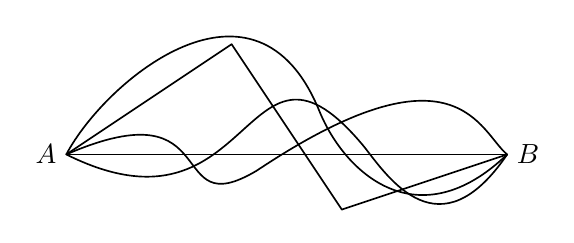
\begin{tikzpicture}[>=latex,scale=0.7]
  \useasboundingbox(-4.7,-1.1)rectangle(4.7,2.3);
  \tkzDefPoints{-4/0/A, 4/0/B, -1/2/C, 1/-1/D}
  % \tkzDrawPoints[fill=black](A,B,C,D,E)
  \tkzDrawSegments[semithick](A,B A,C C,D D,B)
  \draw[semithick](A)..controls(-3.274, 1.368)and(-0.555, 3.600)..( 0.591, 0.790)..controls( 1.057,-0.352)and( 2.385,-1.546) ..(B);
  \draw[semithick](A)..controls(-1.089, 1.261)and(-2.232,-1.297)..(-0.544,-0.294)..controls( 3.096, 2.134)and( 3.503, 0.402)..(B);
  \draw[semithick](A)..controls(-0.539,-1.723)and(-0.790, 2.793)..( 1.407, 0.137)..controls( 1.846,-0.425)and( 2.767,-1.808)..(B);
  \tkzLabelPoints[left](A)
  \tkzLabelPoints[right](B)
\end{tikzpicture}
\end{document}